\appendix
\renewcommand{\thesection}{APPENDIX \Alph{section}}
\section{ -- Ábrák} \label{appendix:A}
\topskip0pt
\vspace*{\fill}
\begin{center}
    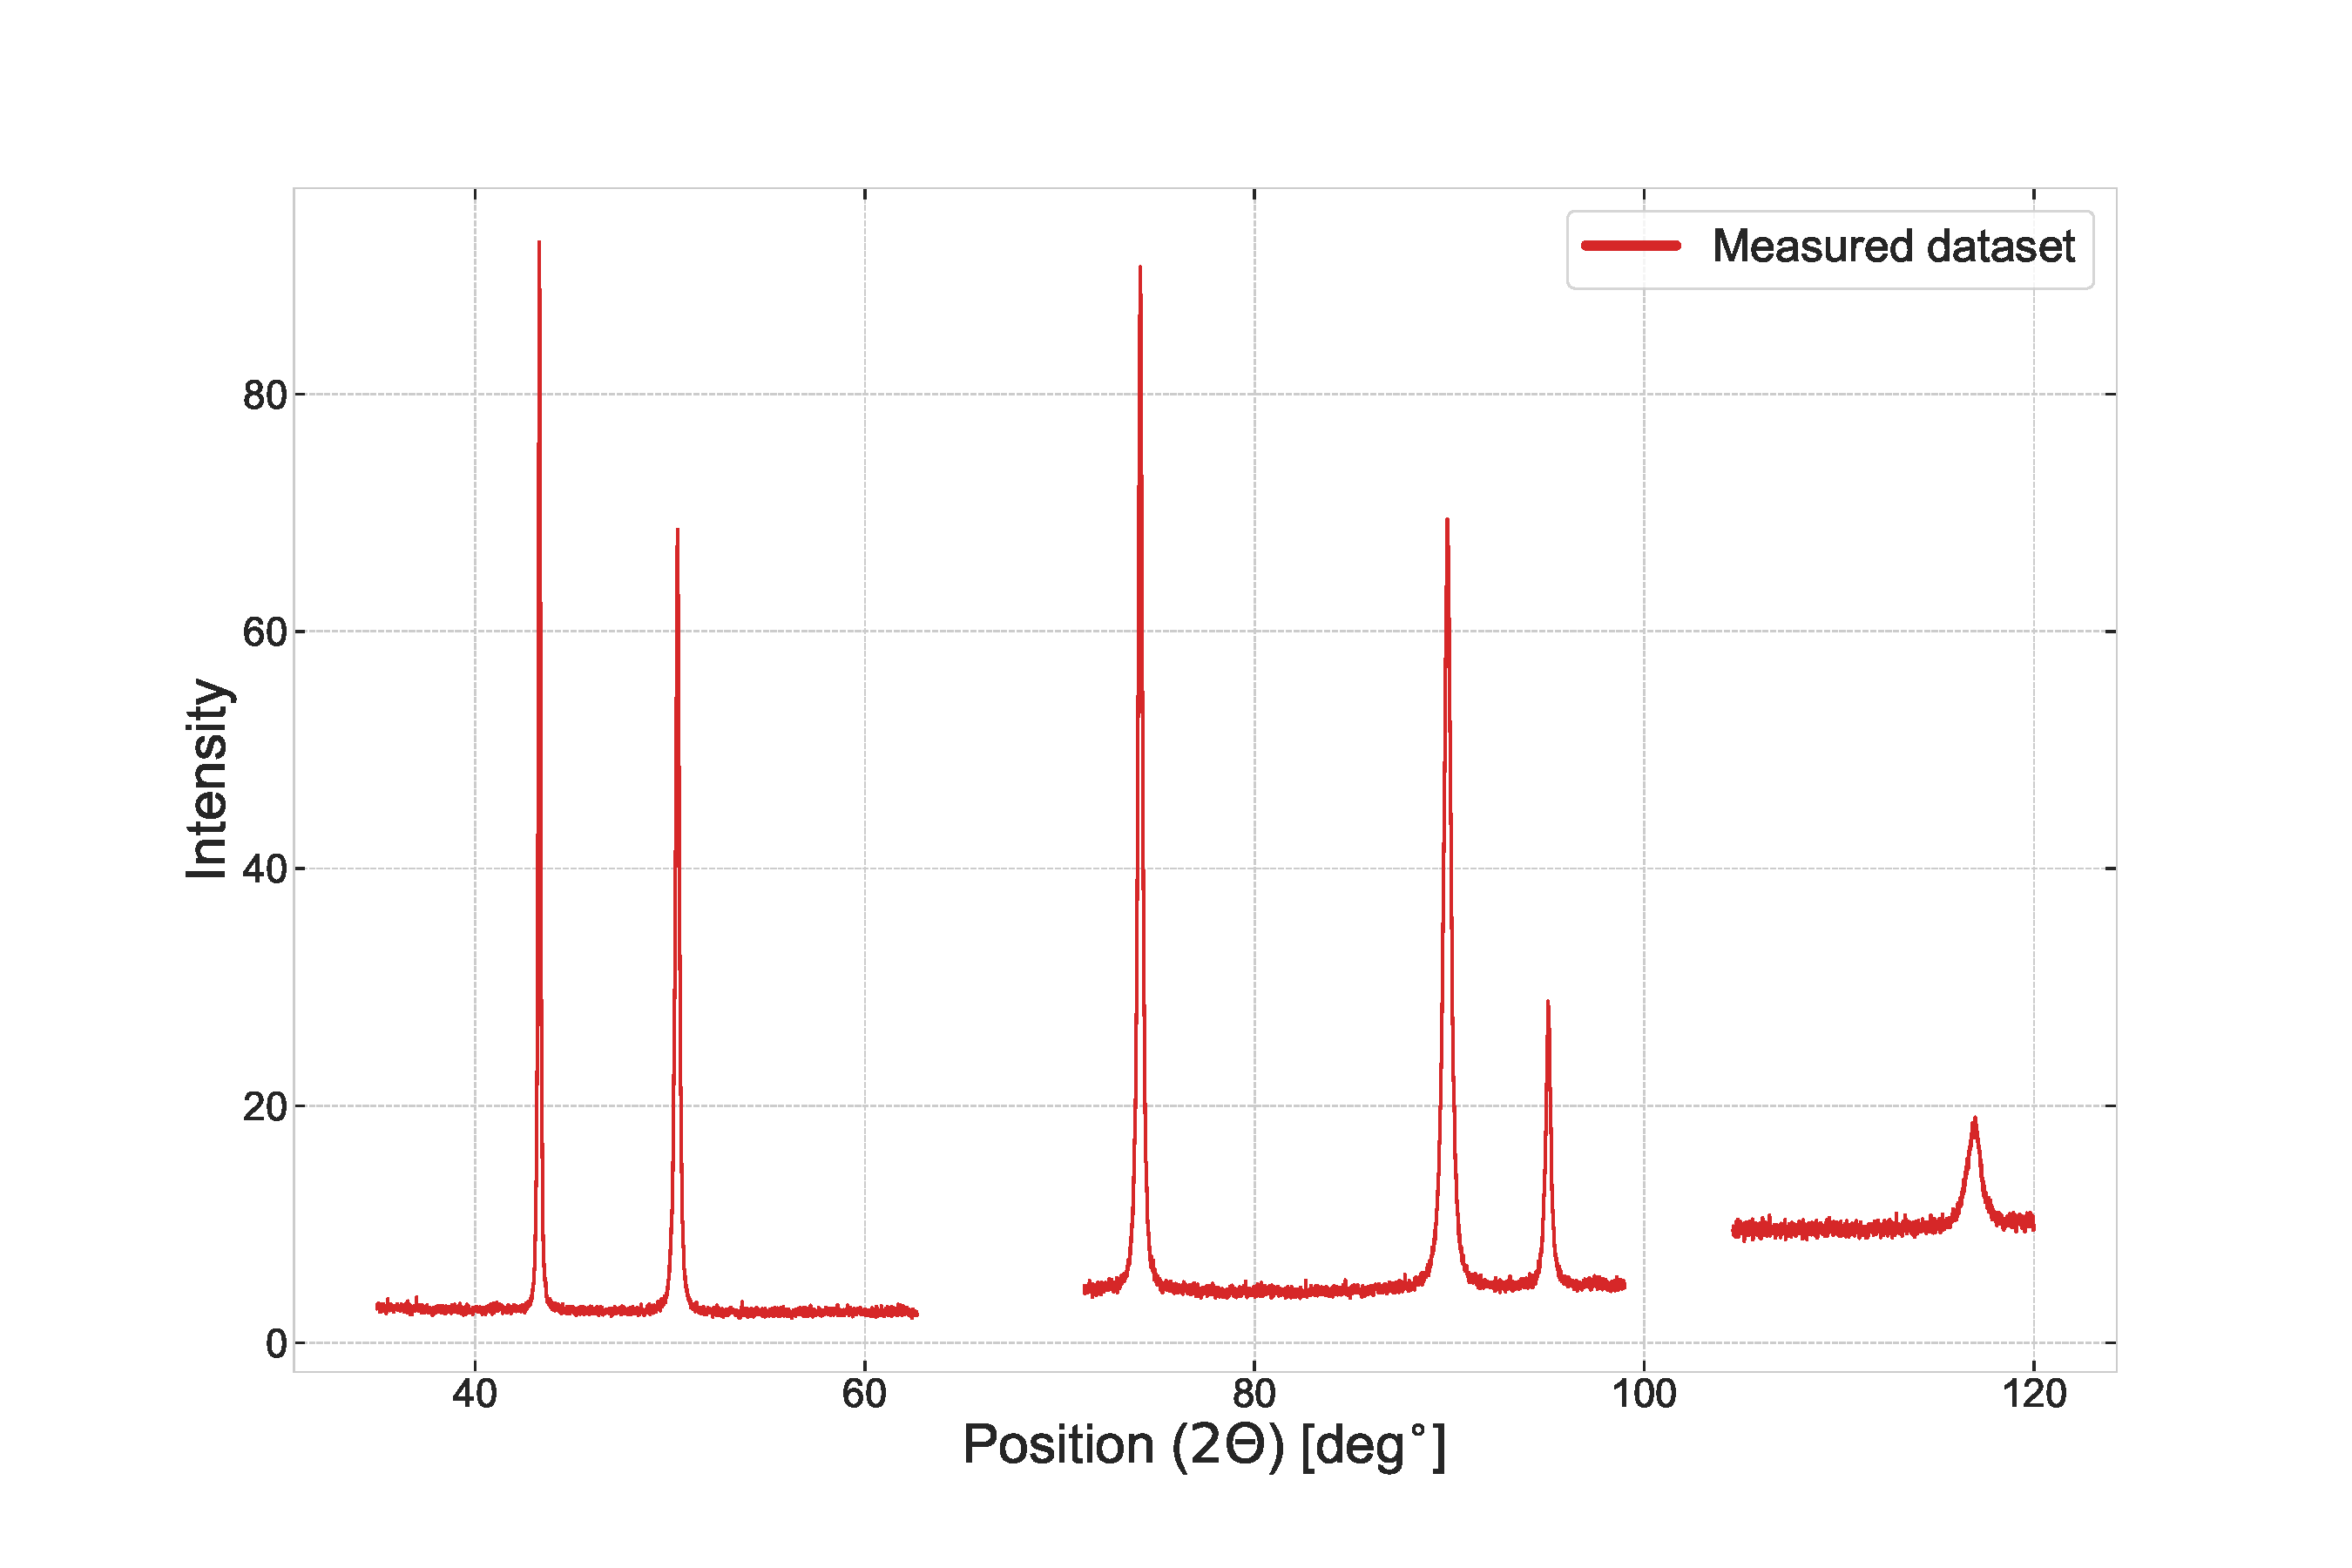
\includegraphics[width=0.9\textwidth]{img_src/measured_data.pdf}
    \captionof{figure}{Az image plate kiolvasása szakaszosan több részletben történt. A kapott individuális képeket az ELTÉ-n megtalálható szoftver segítségével kiértékeltük és belőlük a diffrakciós csúcsok szög-intenzitás függvényét hoztuk létre. Az egyes képekre kapott függvényeket ugyanezzel a programmal összeillesztettük, hogy meghatározhassuk a csúcsok alatti területek méretét.} \label{fig:1}
\end{center}
\begin{center}
    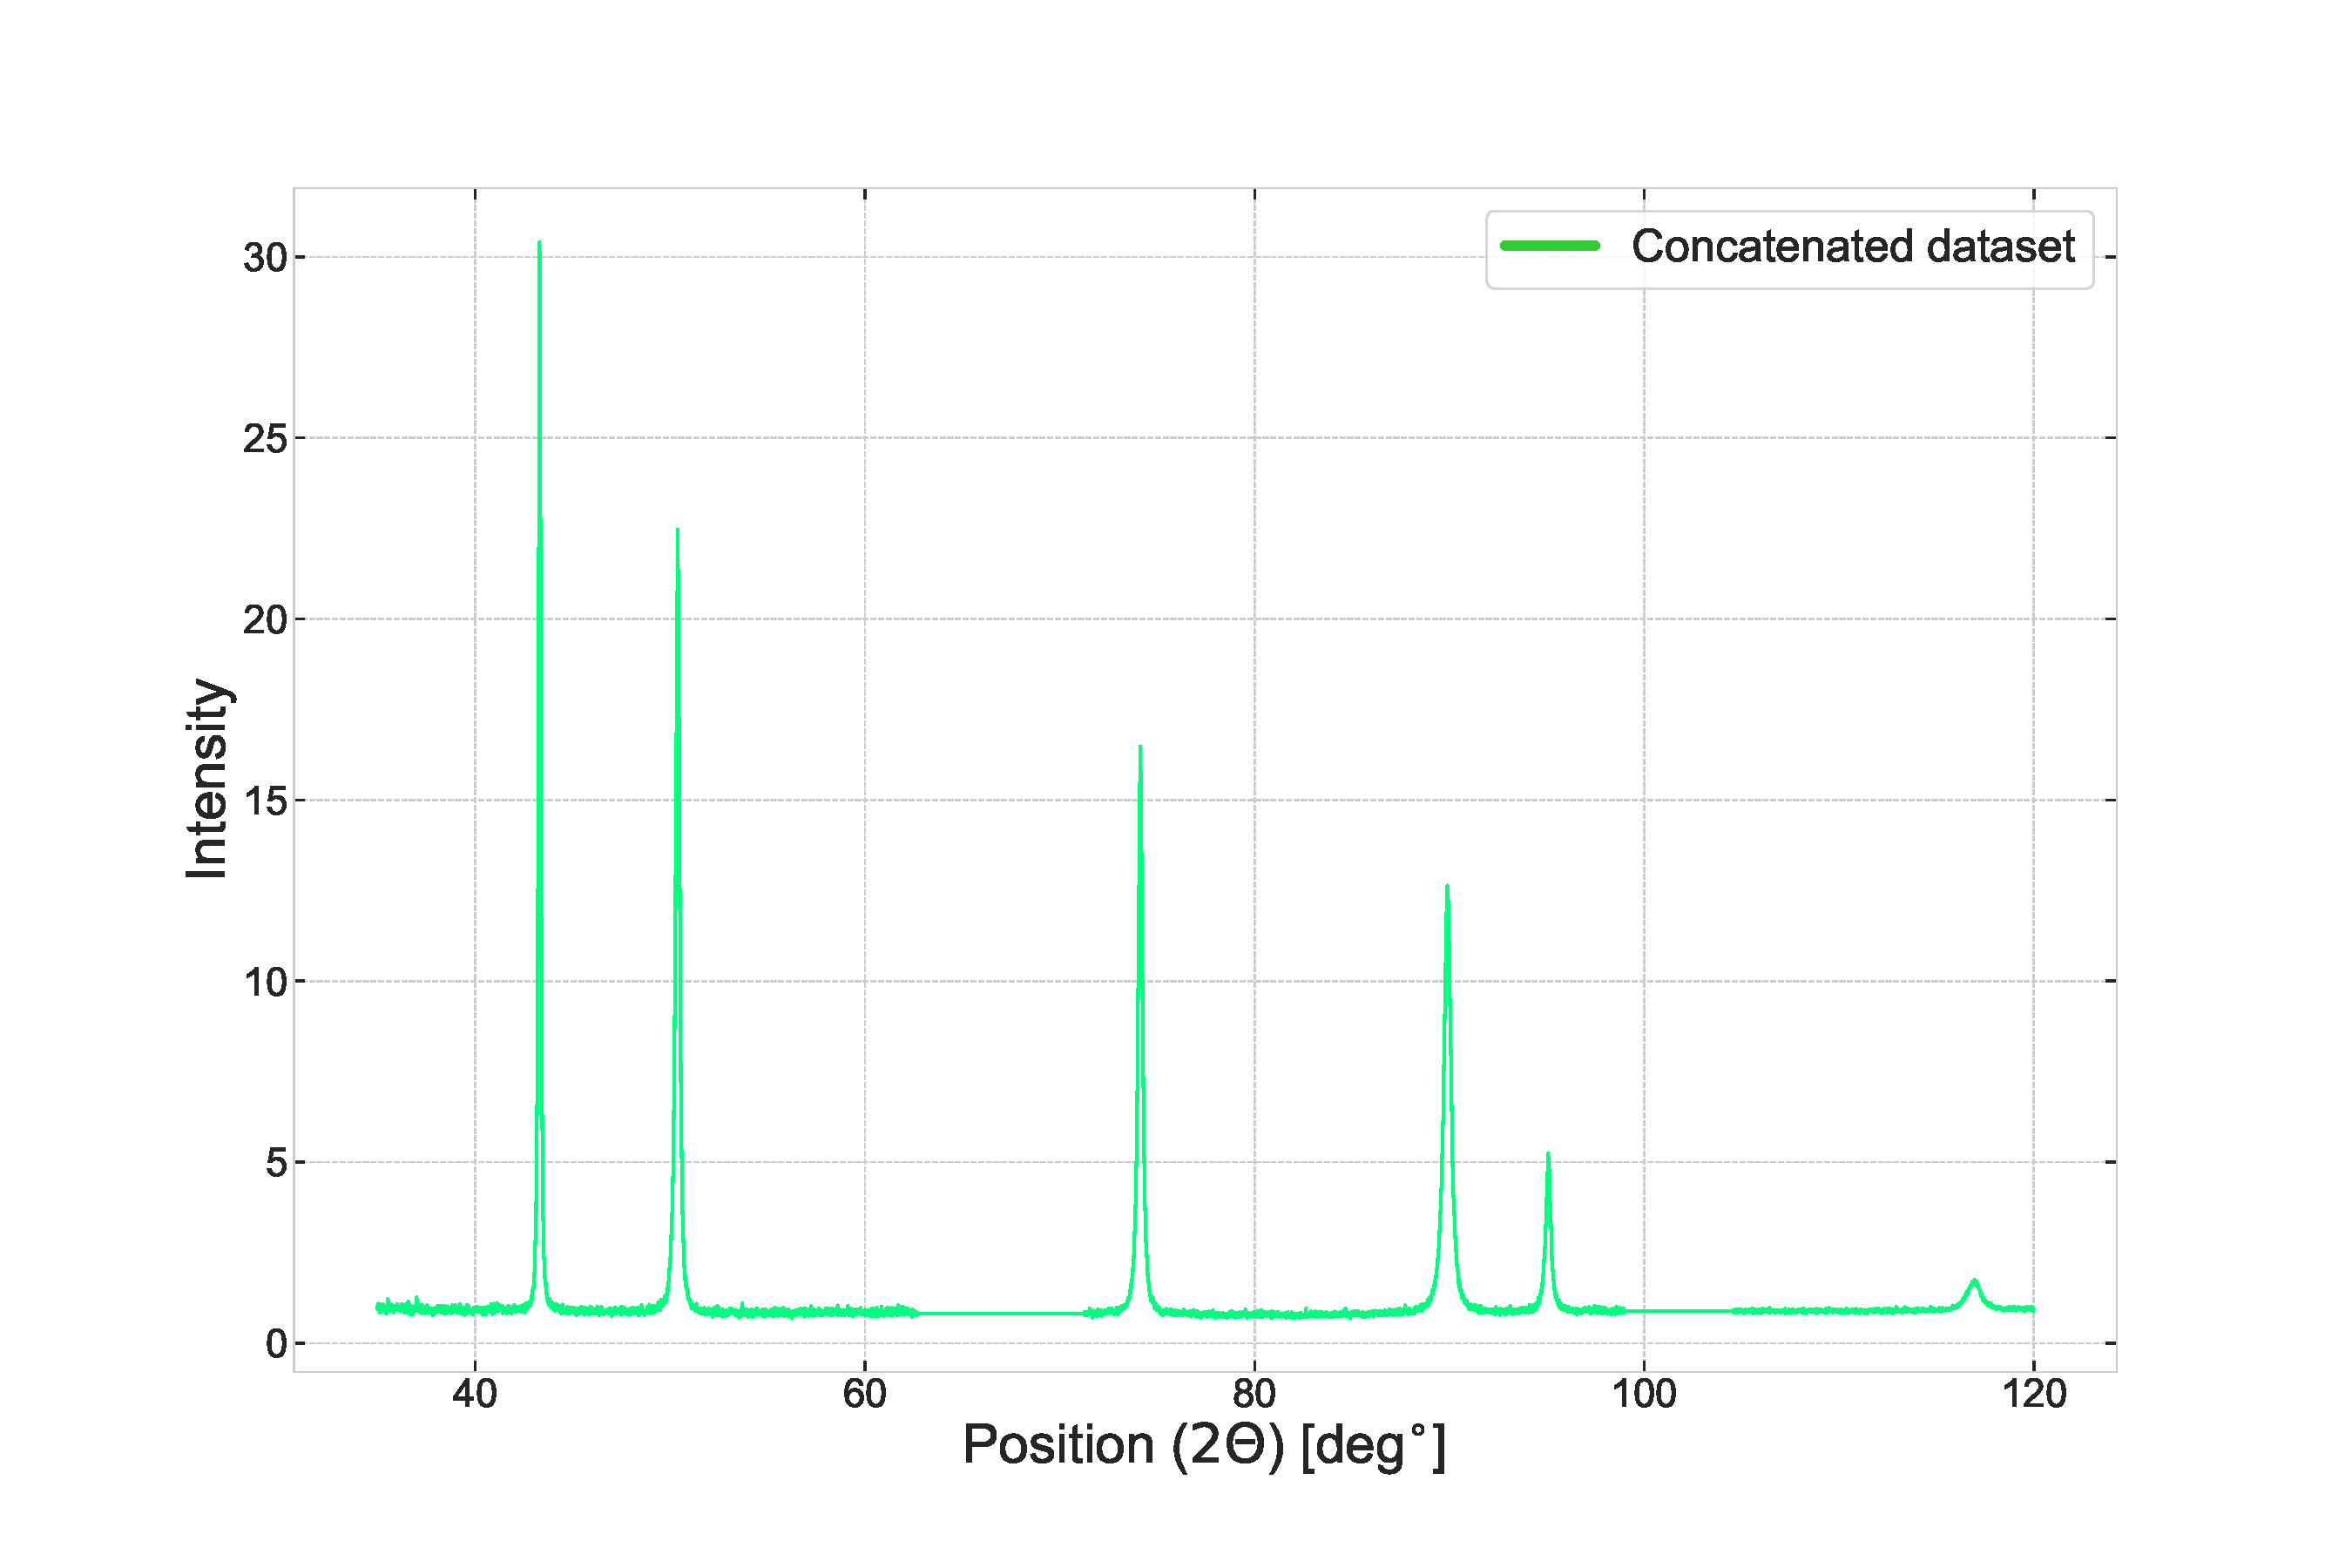
\includegraphics[width=0.9\textwidth]{img_src/prepared_data.pdf}
    \captionof{figure}{Az image plate beolvasásánál kapott 3 különálló szakasza a diffrakciós csúcsok szög-intenzitás függvényének. A szoftveres elemzés többek között ezen szakaszok azonos háttérre történő helyezését végezte el.} \label{fig:2}
\end{center}
\vspace*{\fill}
\newpage
\topskip0pt
\vspace*{\fill}
\begin{center}
    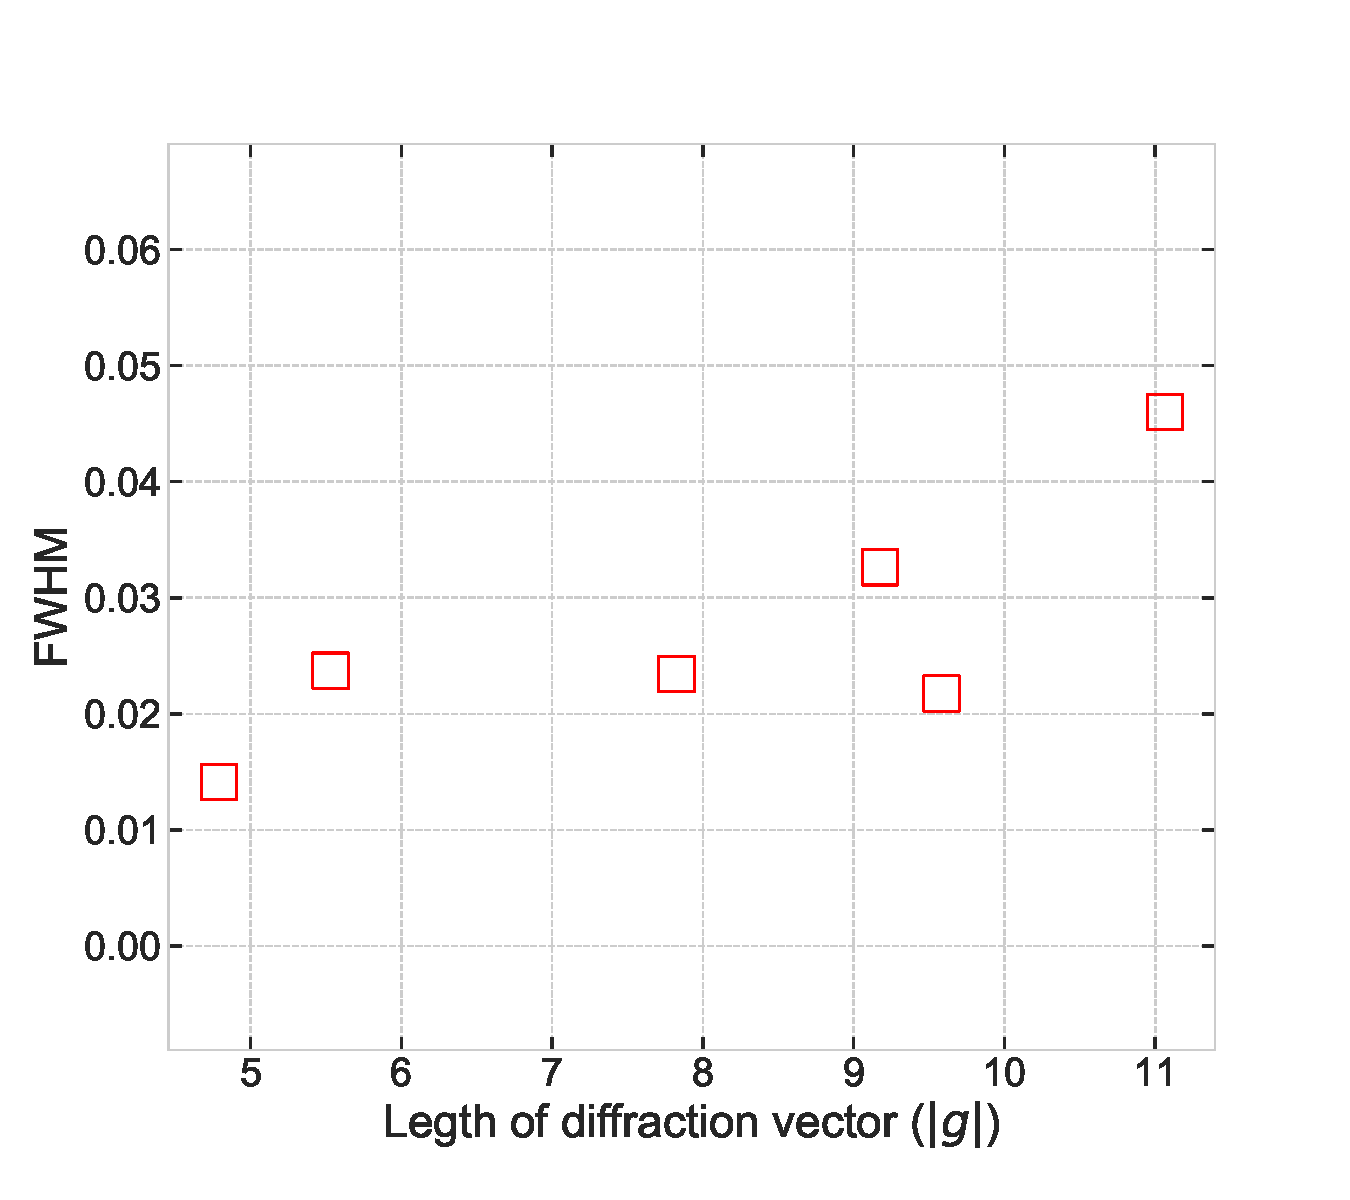
\includegraphics[width=0.7\textwidth]{img_src/williamson_hall.pdf}
    \captionof{figure}{A Cu minta diffrakciós csúcsainak Williamson-Hall ábrázolása a diszlokációk figyelembevétele nélkül.} \label{fig:3}
\end{center}
\begin{center}
    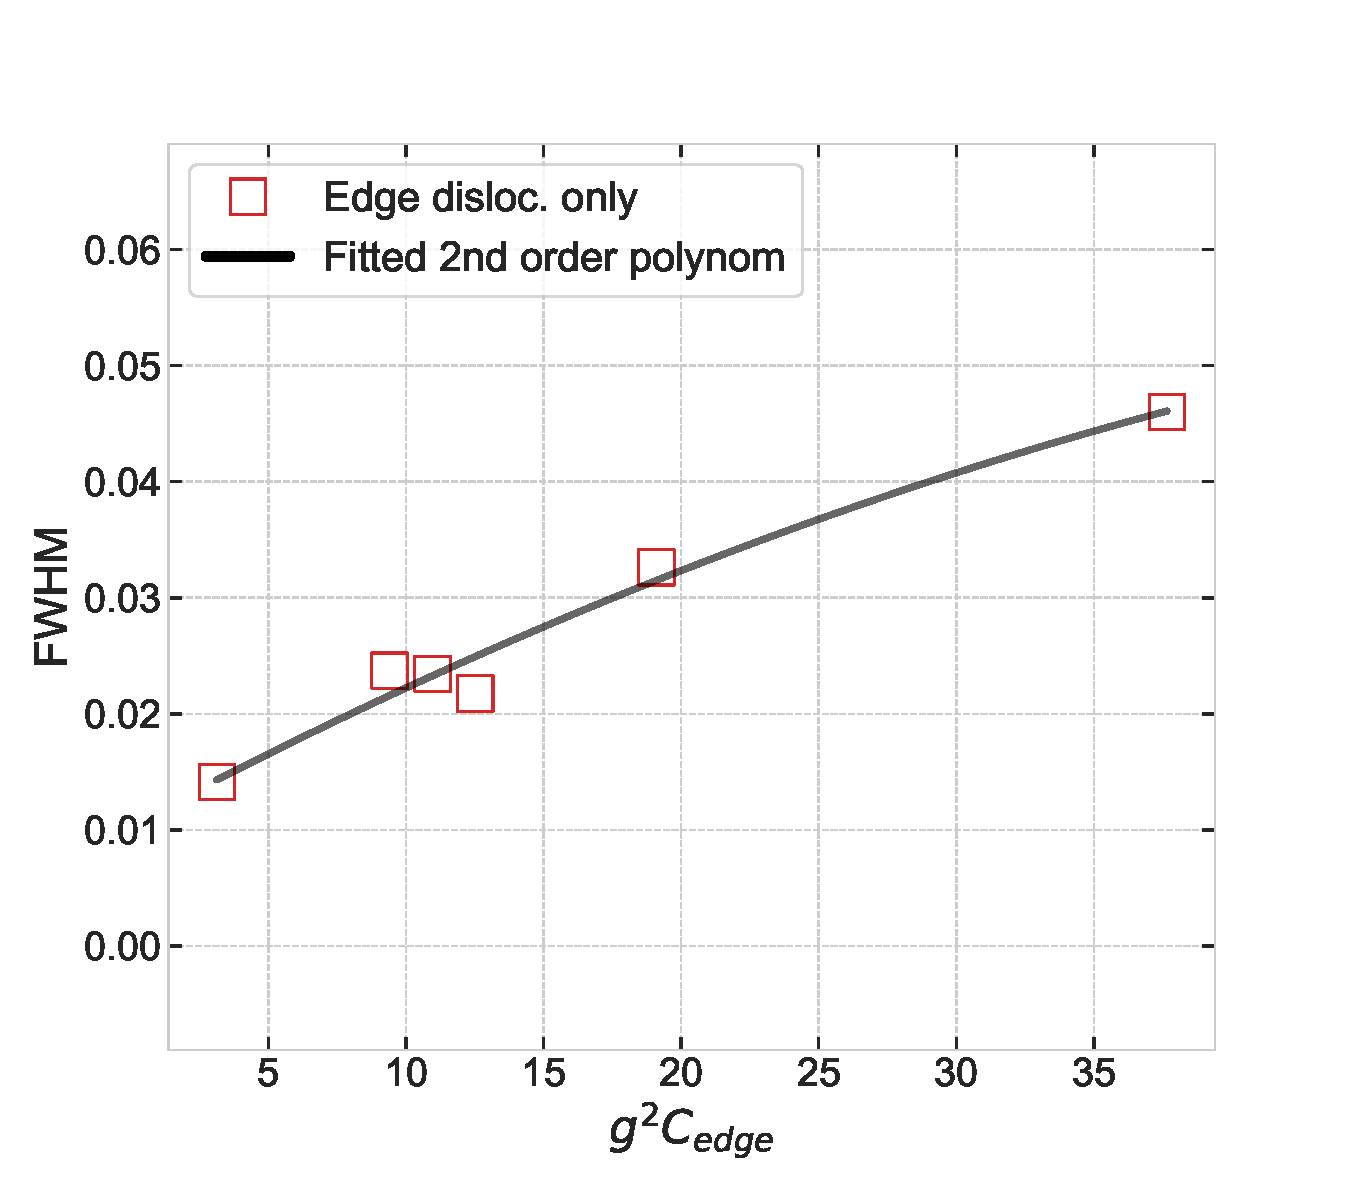
\includegraphics[width=0.7\textwidth]{img_src/williamson_hall_modified_edge.pdf}
    \captionof{figure}{A Cu minta diffrakciós csúcsainak módosított Williamson-Hall ábrázolása, ahol kizárólag az éldiszlokációk hatását vettük figyelembe.} \label{fig:4}
\end{center}
\vspace*{\fill}
\newpage
\topskip0pt
\vspace*{\fill}
\begin{center}
    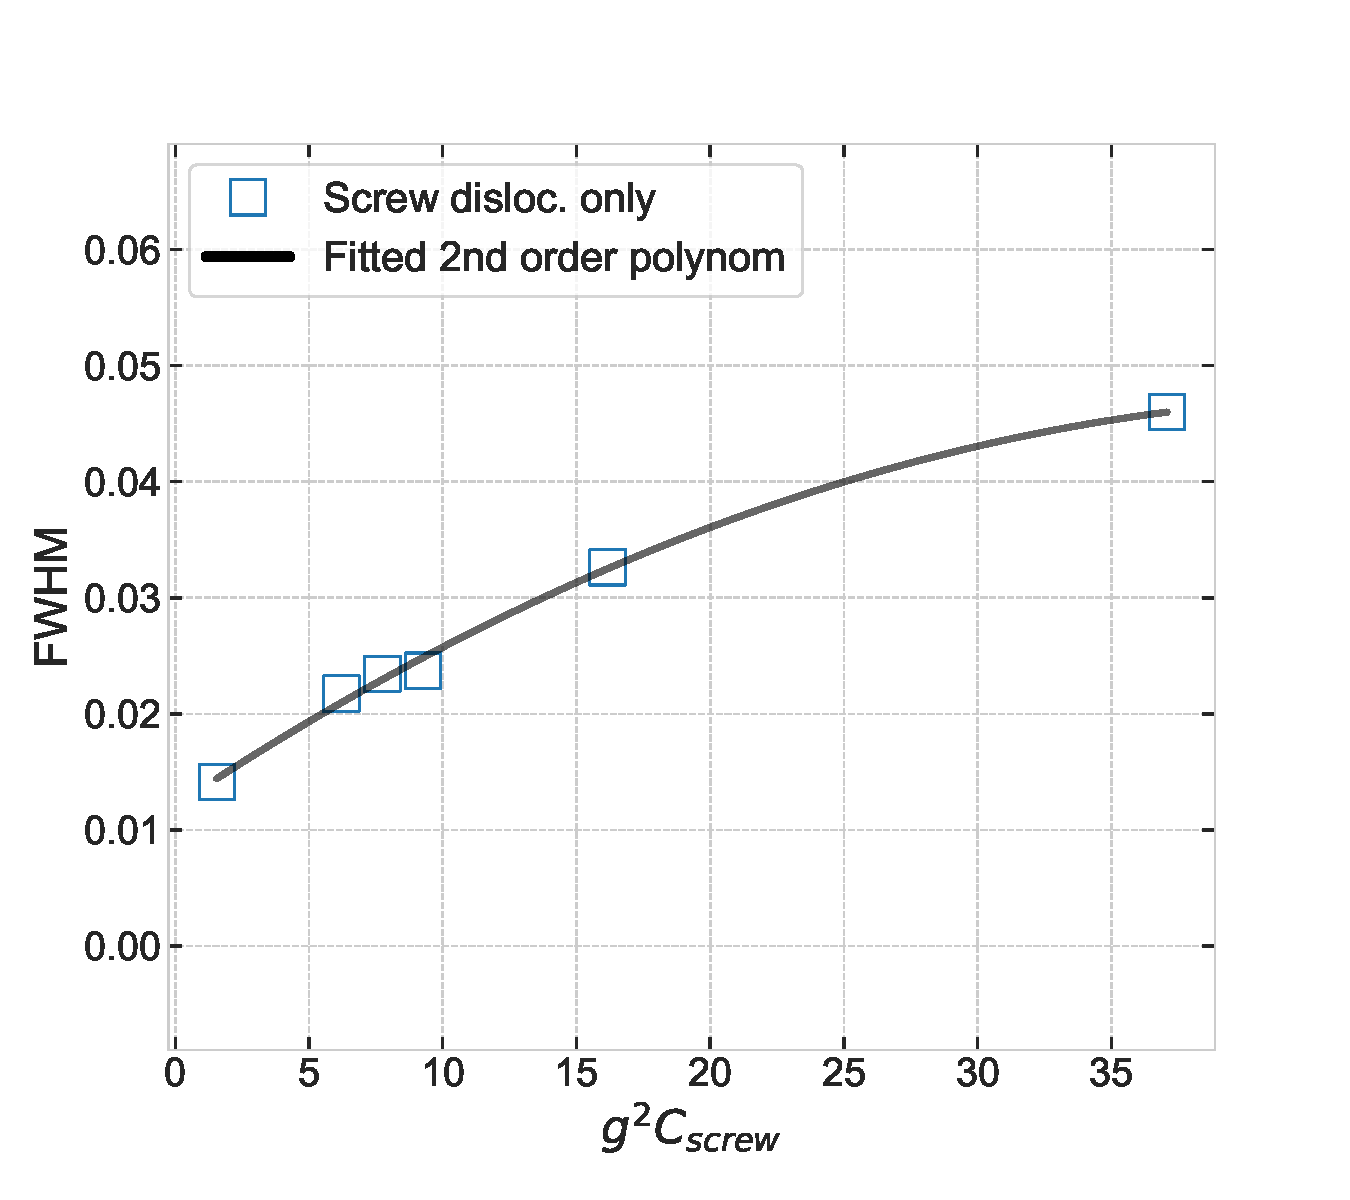
\includegraphics[width=0.7\textwidth]{img_src/williamson_hall_modified_screw.pdf}
    \captionof{figure}{A Cu minta diffrakciós csúcsainak Williamson-Hall ábrázolása, ahol kizárólag a csavardiszlokációk hatását vettük figyelembe.} \label{fig:5}
\end{center}
\begin{center}
    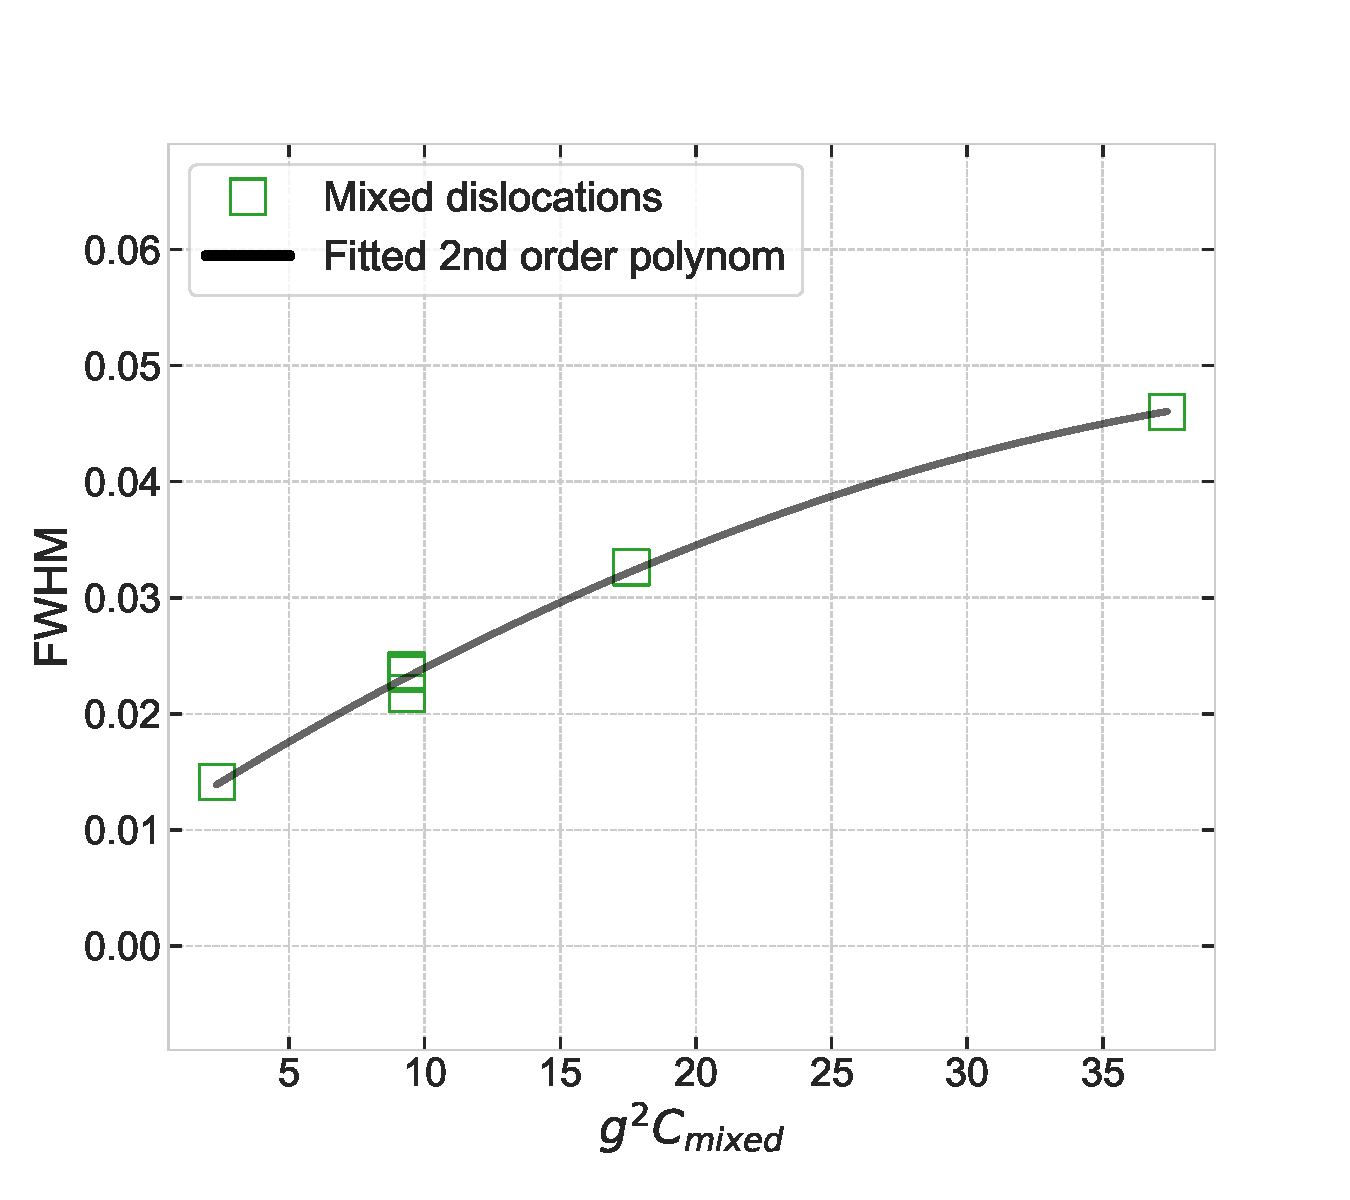
\includegraphics[width=0.7\textwidth]{img_src/williamson_hall_modified_mixed.pdf}
    \captionof{figure}{A Cu minta diffrakciós csúcsainak módosított Williamson-Hall ábrázolása, ahol az él-, valamint a csavardiszlokációk hatásának átlagát vettük figyelembe.} \label{fig:6}
\end{center}
\vspace*{\fill}
\newpage
\topskip0pt
\vspace*{\fill}
\begin{center}
	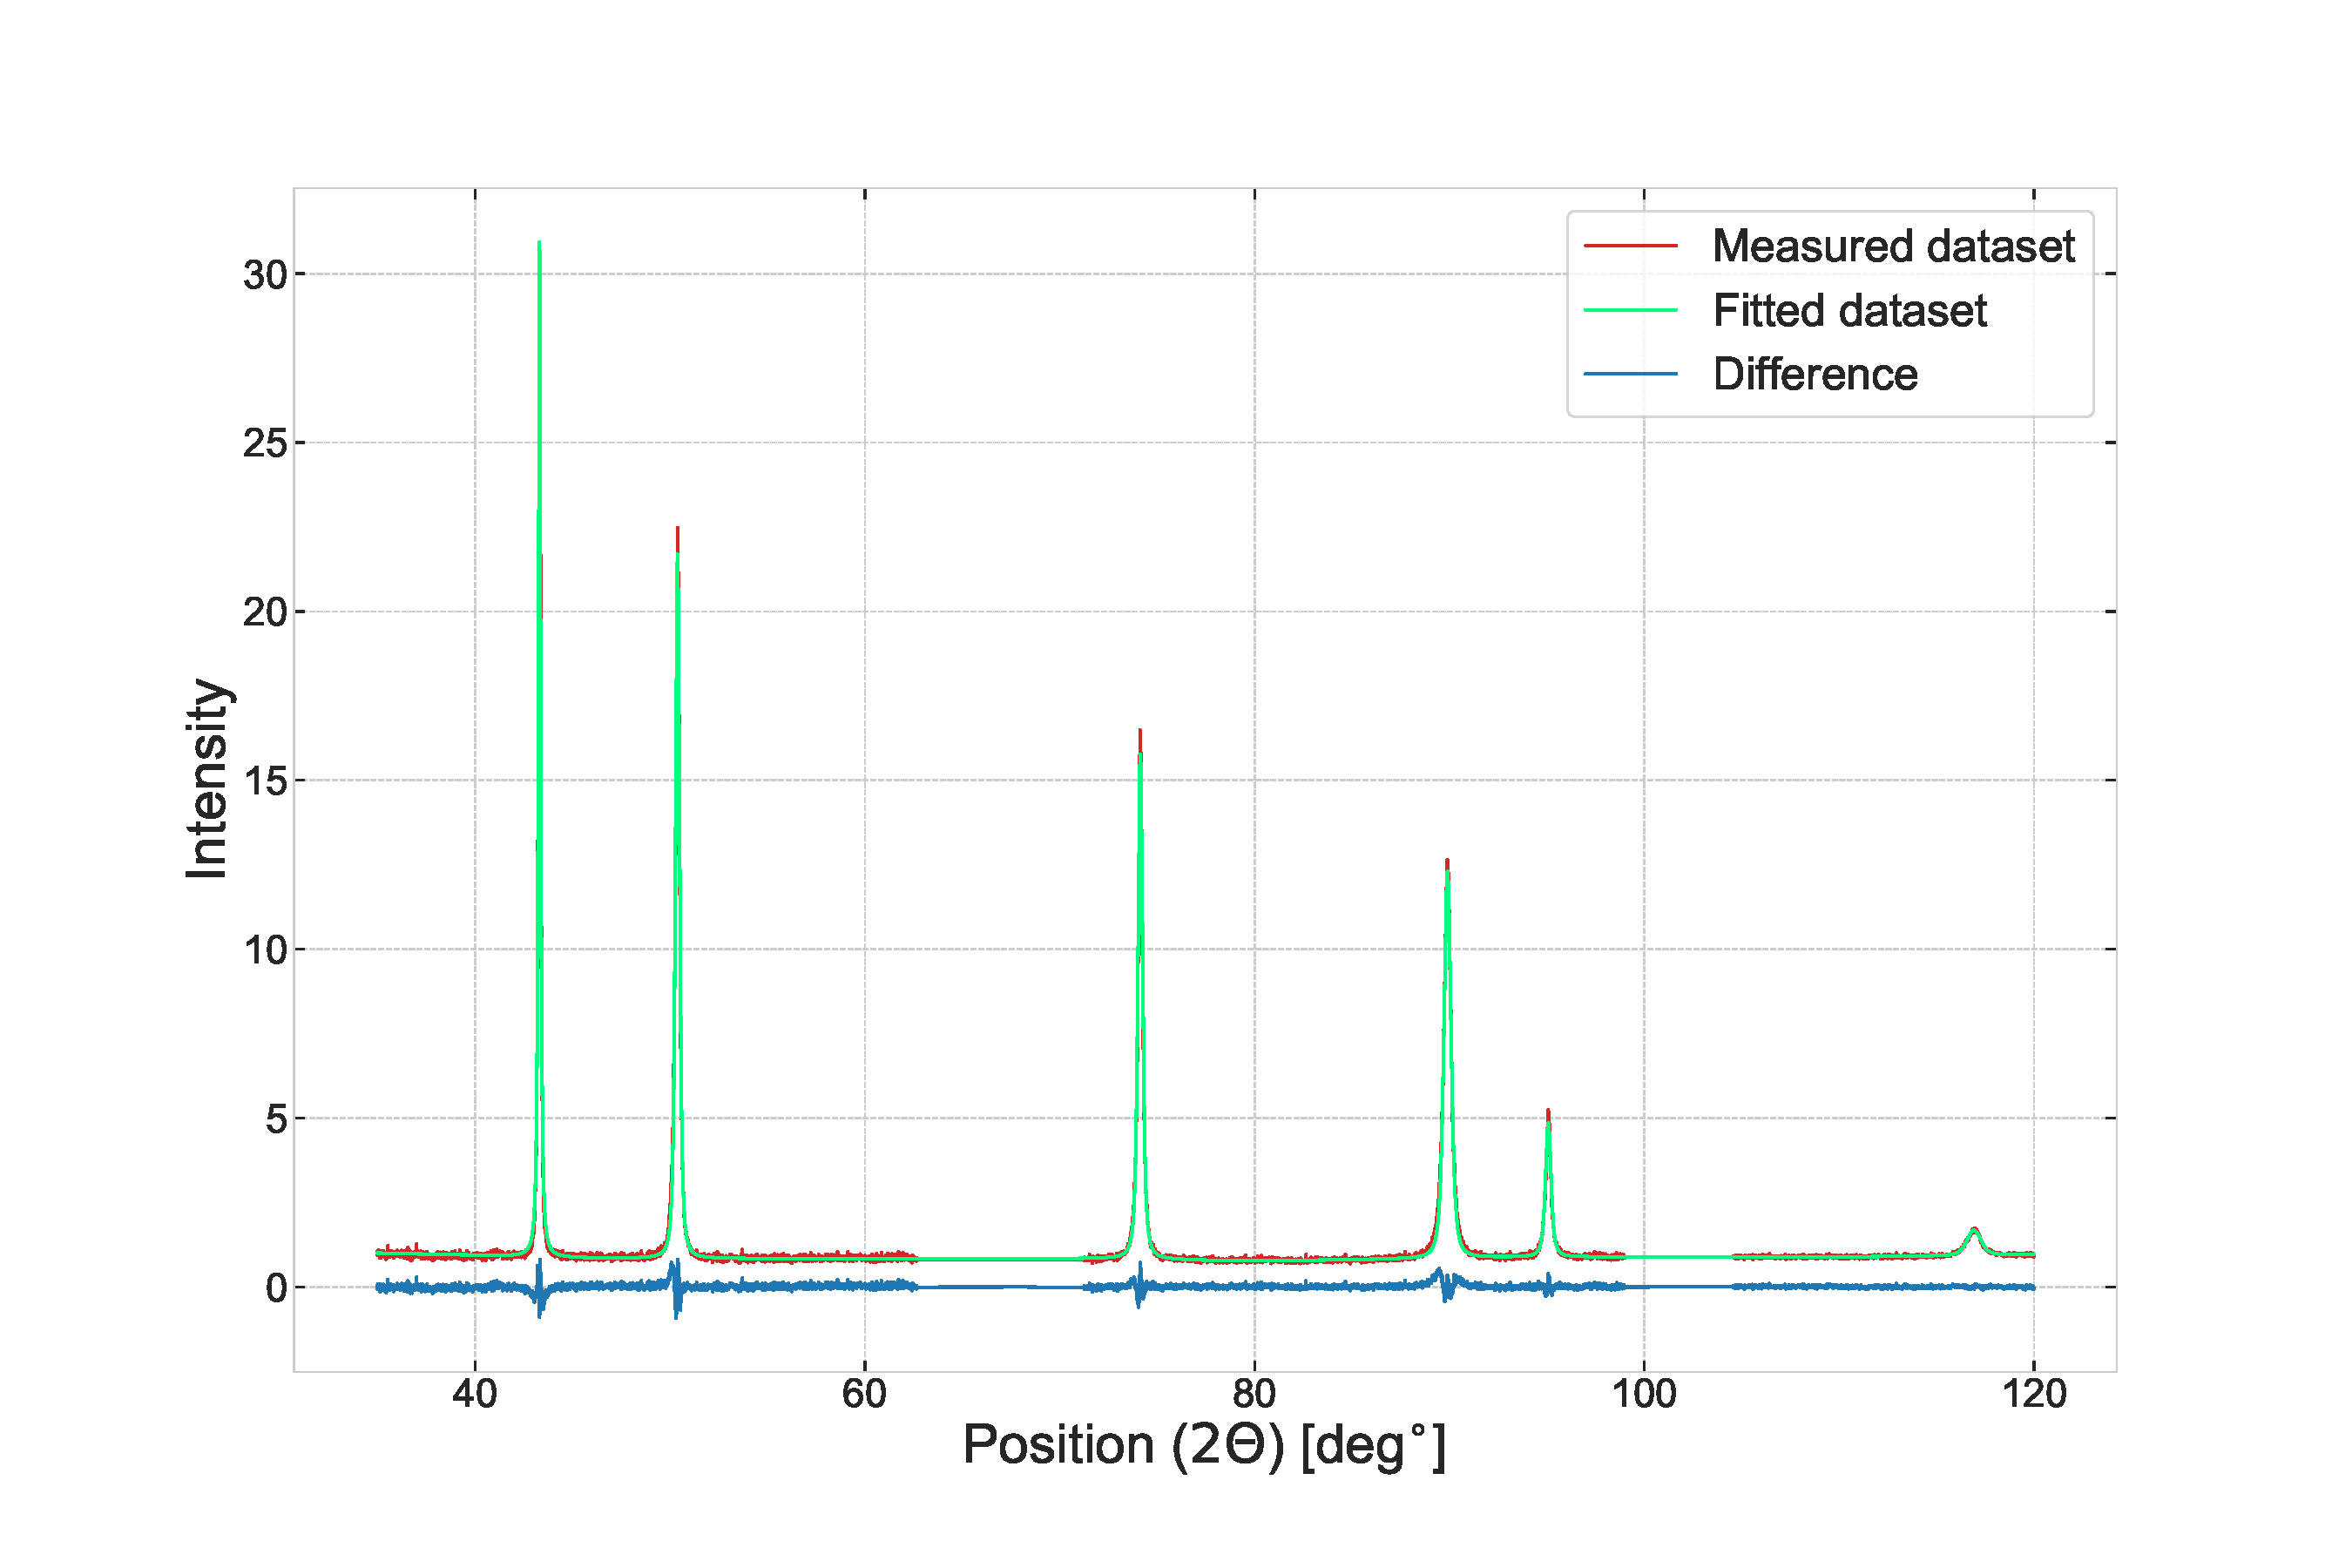
\includegraphics[width=\textwidth]{img_src/CMWP_fit.pdf}
	\captionof{figure}{A CMWP módszer által a mért adatsorra illesztett elméleti profil és a kettő görbe különbsége.} \label{fig:7}
\end{center}
\begin{center}
	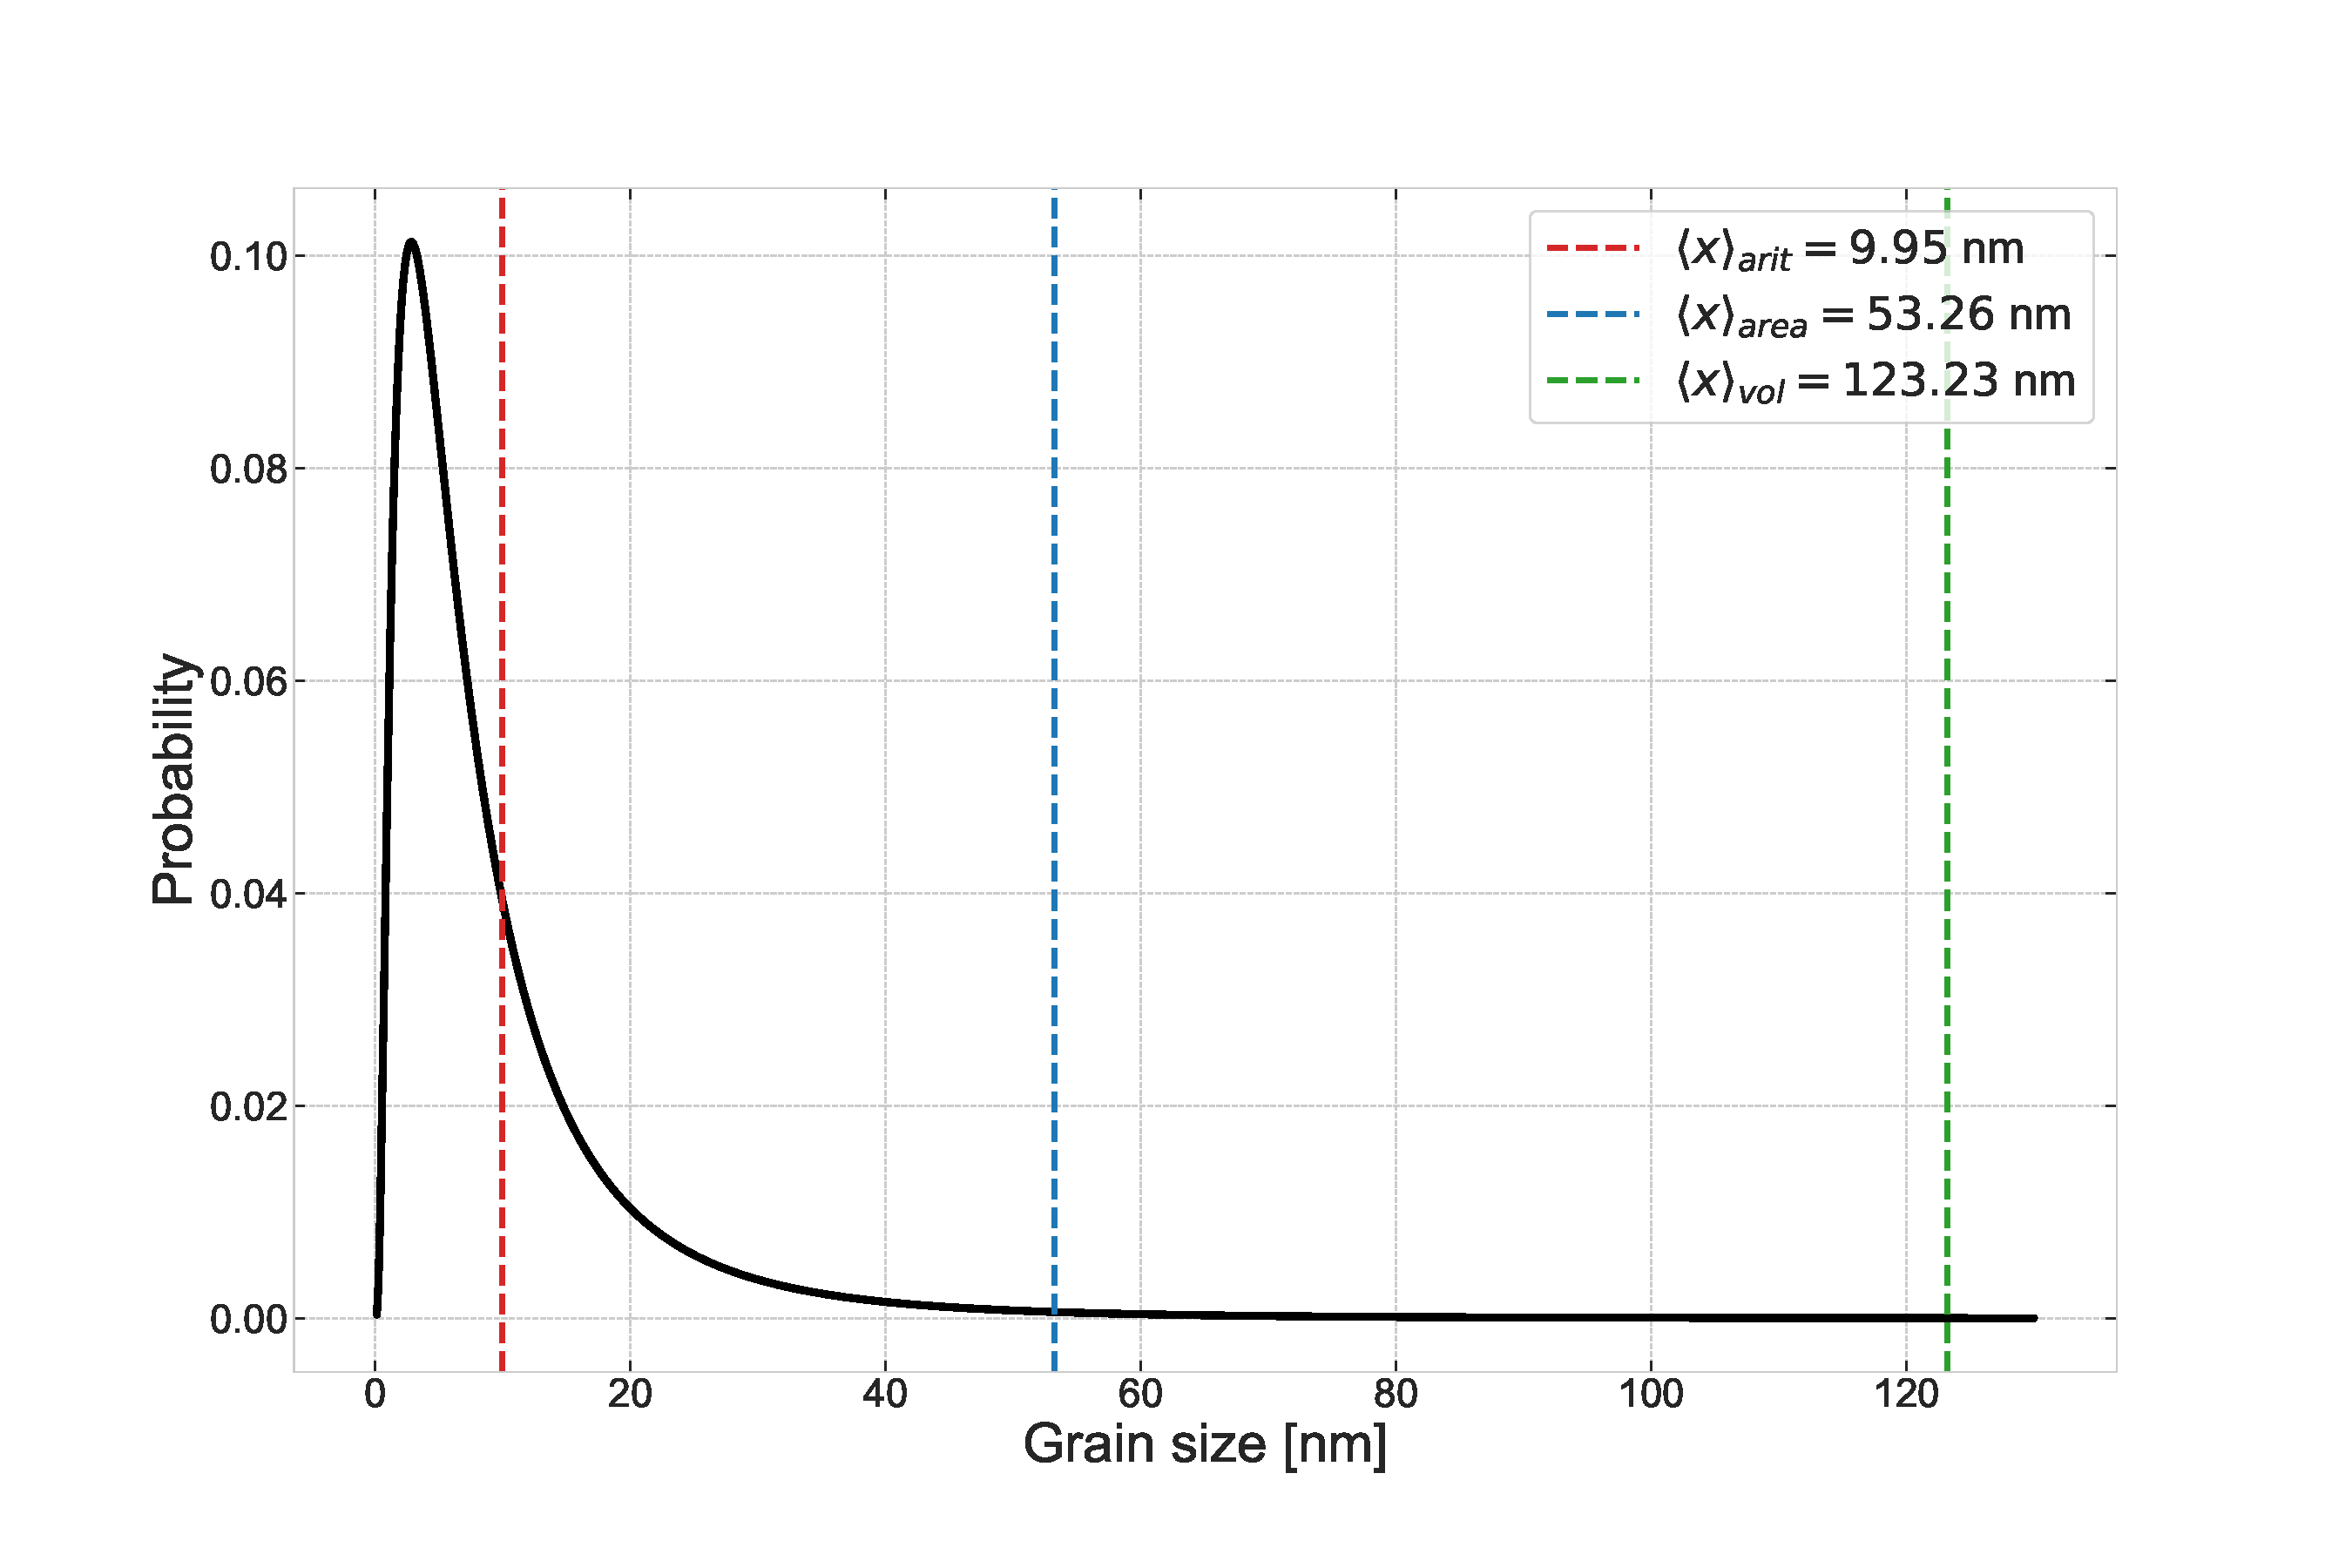
\includegraphics[width=\textwidth]{img_src/CMWP_lognorm.pdf}
	\captionof{figure}{A szemcseméret lehetséges értékei, log-normális eloszlást feltételezve.} \label{fig:8}
\end{center}
\vspace*{\fill}